\documentclass[12pt,twoside,a4paper]{report}

\usepackage[utf8]{inputenc}
\usepackage[T1]{fontenc}


\usepackage{amsmath,amsfonts,amssymb}
\usepackage{graphicx}
\usepackage{float}
\usepackage[lined,boxed,commentsnumbered]{algorithm2e}

\usepackage[usenames, dvipsnames]{color}
\usepackage{fancyhdr}
\usepackage[toc,page]{appendix}


\title{Title to find ...}
\author{Gautier VAILLANT}

\fancypagestyle{newstyle}{
\fancyhf{} % clear all header and footer fields
\fancyhead[l]{\bfseries \nouppercase \rightmark} % except the center
\fancyfoot[R]{\thepage} % except the center
\renewcommand{\headrulewidth}{0pt}
\renewcommand{\footrulewidth}{0pt}}

\pagestyle{newstyle}

\begin{document}

\maketitle

\chapter*{Acknoledgements}

I would first like to gratefully thank Helmut Grubmüller and Bert De Groot for welcoming me in their lab. I also thank Carsten Kutzner who supervised my Internship. I also would like to Thank Bartosz Kohnke and Thomas Ullmann for providing me advice on my project.\\ 

Finally I would also like to thank Ivo Kabadschow and Andreas Beckmann who welcomed me in the Jülich Forschungszentrum to teach me the details of the FMM method. 


\chapter*{Abstract}

Simulating large pairwise interactions is a very important issue for Scientific research. It plays an important role in Astrophysics to know the dynamics of galaxies, in plasma physics or in our case in biophysics. This kind of simulations is typically with a complexity of $\mathcal{O}(N^2)$ which scales badly with the size of the system.

Some other techniques, such as the PME (Particle Mesh Ewald) and the FMM (Fast Multipole Method) are able to obtain a complexity of respectively $\mathcal{O}(N\log(N))$ qnd $\mathcal{O}(N)$.
\\
\\
\\
\\

La simulation de larges systemes de particules en interaction est tres importante pour le calcul scientifique. Elles jouent un role important en Astrophysique pour connaitre la dynamique des galaxies, en physique des plasmas ainsi que, dans notre cas, en Biophysique.


\tableofcontents

\chapter*{Presentation of the Lab}
\chapter*{Context of the Internship}

The Context of this Internship is driven by the "SPPEXA (Software for exascale computing) / GromEx" project funded by the DFG (Deutsche Forschungsgeimeinschaft).
The Idea of this project is to create a flexible and fast solver for computing forces and potentials, which is a preliminary for molecular simulations.

A poster\footnote{from http://www.mpibpc.mpg.de/grubmueller/sppexa}   of the project can be found below :

\begin{figure}[H]


\includegraphics[scale=2]{sppexa-poster}
 \centering
 
\caption{Poster for the SPEXXA project}

\label{fig:poster}

\end{figure}


Currently the method used for computing electrostatic forces is called the PME (Particle Mesh Ewald). It works nicely but one of its problems is that the algorithms cannot br efficiently parallellised tasks as there is a lot of communication between the CPU and GPU cores. The idea would be to replace this method with a new method called the Fast-Multipole Method which is based on a tree Structure and may allow an greater parralilization of the system as wanted.\\

So the Idea of the Internship is first to know if the both method method have the same accuraracy and for which parameters.


\chapter{Methods for computing electrostatic forces}


\section{$\mathcal{O}(N^2)$ method }


In this section, we will explain the most basic method to compute pairwise interactions and explain why the method leads to longs computation times and sometimes artifacts.

\subsection{Naive Method}

The coulombic interaction between two charged particles can be written the following way:

\begin{equation}
	\overrightarrow{F}_{A \rightarrow B} = \frac{q_A q_B \hat{r}_{AB} }{4\pi\epsilon_0|R_{AB}|^2}
	\label{coulombComplete}
\end{equation}

where $q_A $ and $q_B$ are respectively the charges of A and B, ansection{Possible improvements}d $R_{AB}$ is the distance between $A$ and $B$.

In the thesis we will simplify the units of ~\eqref{coulombComplete} for computational reasons by just writing :

\begin{equation}
	\overrightarrow{F}_{A \rightarrow B} = \frac{q_A q_B \hat{r}_{AB} }{|R_{AB}|^2}
	\label{coulombSimplified}
\end{equation}

The Corresponding potential for a charged particle, with a charge $q$ is :

\begin{equation}
	V = \frac{1}{r}
	\label{potential}
\end{equation}



The first, naive way to compute electrostatic forces is the following : in order to compute the force acting on one particle, it is needed to obtain the coulombic interaction for each pair of particles.

So if we consider a set of $N$ charged particles, $N-1$ interactions are needed to compute the force acting on one specific particle. So in order to know the forces of the set of particles, $N\cdot(N-1)$ operations are needed, hence an algorithmic complexity of $\mathcal{O}(N^2)$.

This gives the following algorithm:



\IncMargin{1em}
\begin{algorithm}[H]

\SetKwData{Left}{left}\SetKwData{This}{this}\SetKwData{Up}{up}
\SetKwData{Force}{force}

\SetKwFunction{ComputeForce}{computeForce}
\SetKwFunction{Union}{Union}\SetKwFunction{FindCompress}{FindCompress}
\SetKwInOut{Input}{input}\SetKwInOut{Output}{output}

\Input{A set of $N$ charged Particles}
\Output{A List of the forces
for each particle}
\BlankLine

\emph{For each particle i}\;
\For{$i\leftarrow 1$ \KwTo $N-1$}{
\emph{add interaction between particle $i$ and particle $j$ }\;
\For{$j\leftarrow i+1$ \KwTo $N$}{

	\Force$[i]$  $\leftarrow$ \Force$[i]$ + \ComputeForce{$i,j$}   \;

}
}
\caption{Naive method}\label{algo_disjdecomp}
\end{algorithm}\DecMargin{1em}


The complexity of such a computation limits its use to rather small systems and is not really usable for bigger systems such as proteins or astrophysical systems.


\subsection{Possible improvements}

A possible improvement is to limit the interaction to a certain radius : if the distance between two particles if greater tham $R_0$, then the force is set to $0$.

So we have the following system :


\begin{equation}
  \overrightarrow{F}_{A \rightarrow B}  =
	\begin{cases}
	  \frac{q_A q_B \hat{r}_{AB} }{|R_{AB}|^2}  & \text{if } R_{AB} < R_0 \\
	  \overrightarrow{0} & \text{otherwise}
	\end{cases}
\end{equation}

This technique is for example used for Lennard-Jones potentials ($V_{LJ} = 4\epsilon [(\frac{\sigma}{r})^12 - (\frac{\sigma}{r})^6] $), where the Intensity of the force is quickly decreasing. It allows to limit the number of interactions to only the close neighbours.\\

However, one of the problems of this optimisation, especially for long-range interactions such as coulombic interactions is that using a cut-off can lead to artefacts : A particle feels the force, then crosses the cut-off radius. Suddenly, the particle doesn't feel any force anymore, thus the artefacts as it is showed figure \ref{fig:artefact} .

\begin{figure}[H]

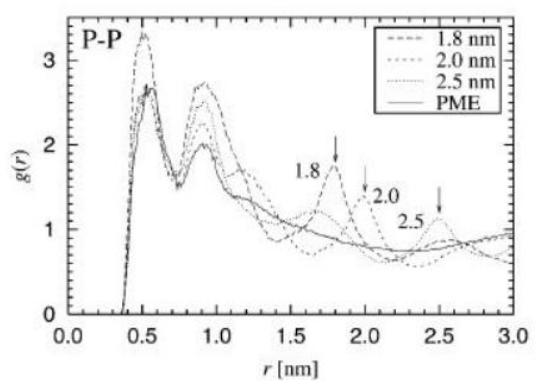
\includegraphics[scale=0.8]{artefact}
 \centering
 
\caption{Radial distribution function (RDF) $g(r)$ between the two
central atoms in the headgroup of a molecule: Cutoff distances are indicated by arrows. from [ADD REFERENCE]}

\label{fig:artefact}

\end{figure}


As we can see in figure \ref{fig:artefact},  the radial distribution of the distance between two atom shows a peak, corresponding to the cutoff of the system. This shows that by using a cut-off technique we might see some artefacts.\\

So the two reasons we don't use a $\mathcal{O}(N^2)$ method is first because of its complexity, and using some optimization techniques can also lead to artifacts.



%-------------------------------------------------------------------------------------------


\section{Fourier Transform-Based methods}

In this section, we will explain techniques using periodic boundary conditions and Fourier transformation in order to compute the potentials and the forces of the particles.

\subsection{Ewald Summation}

This subset of techniques comes from a theoretical physics technique called the Ewald summation.

Using periodic boundary conditions, the potential $V$ of one particle of the system is:

\begin{equation}
	V = \sum_{n_x,n_y,n_z} \sum_{i}^{N} \sum_{j}^{N} \frac{q_i q_j}{r_{ij}}
	\label{periodicSum}
\end{equation}
where $n_x,n_y,n_z$ are the box index vector.\\

The equation \ref{periodicSum} is conditionally convergent and slow to converge. One technique discovered by Ewald is to split the potential in two absolutely convergent terms and one constant term:


If the system is neutral, ie. $\sum_{i=1}^N q_i = 0$, The idea is to split the potential the following way :

\begin{equation}
    V = \frac{1}{r} = \frac{f(x)}{r} + \frac{1 - f(x)}{r}
\end{equation}


\begin{equation}
    V = V_{\text{direct}} + V_{\text{reciprocal}}
\end{equation}

We want to choose $f$, so that $\frac{f(x)}{r}$ is quickly decaying and $\frac{1 - f(x)}{r}$ is as smooth as possible. In this decomposition $\frac{f(x)}{r}$  is as small as possible, even $0$ above a certain cut-off. Then, $\frac{1-f(x)}{r}$ is smooth enough so we can compute its Fourier transform with just a few $\overrightarrow{k}$ vectors. This gives a quick computation of the reciprocal space.

a good choice is often $f(x) = \text{erfc}(\alpha x)$, where $\alpha$ is called the splitting parameter, and $\text{erfc}(x) = \frac{2}{\sqrt{\pi}} \int_{x}^{+\infty}{e^{-t^2}\text{dt}} $\\

so we obtain the following potentials :\\

For the direct space :

\begin{equation}
   V_{\text{direct}} =  \frac{1}{2} \sum_{n_x,n_y,n_z} \sum_{i,j}^{N} q_i q_j \frac{\text{erfc}(\alpha r)}{r}
\end{equation}

and for the reciprocal space :

\begin{equation}
\label{Vrecip}
	V_{\text{reciprocal}} = \frac{1}{2 \pi V} \sum_{i,j}^{N} q_i q_j \sum_{n_x^*,n_y^*,n_z^*}\frac{\exp{-(\pi \overrightarrow{m}/\alpha)^2} +2\pi i \overrightarrow{m} \cdot (r_i - r_j)}{m^2}
\end{equation}

where $n_x^*,n_y^*,n_z^*$ are the vectors in the reciprocal space.\\


Once the electrostatic potentials are obtained, it is possible to differentiate the potentials to obtain the force on each particle.\\

let $p = (x,y,z)$ a coordinate of the system, then :


\begin{equation}
   \overrightarrow{F}_p^{\text{direct}} = \overrightarrow{\nabla}_p V_{\text{direct}} 
\end{equation}


so we have:

\begin{equation}
\label{ewaldDirect}
   \overrightarrow{F}_p^{\text{direct}} = q_i \sum\limits_{i=1,i\neq j}^N \sum\limits_{\textbf{n}} q_j \frac{(r_{ij,n})_p}{r_{ij,n}^3}
   \{\text{erfc}(\alpha (r_{ij,n}) + \frac{2\alpha}{\sqrt{\pi}} r_{ij,n} \exp(-(\alpha r_{ij,n})^2)\}
\end{equation}


\begin{equation}
\label{ewaldReciprocal}
   \overrightarrow{F}_p^{\text{reciprocal}} = \frac{2 q_i}{L} \sum\limits_{i=1,i\neq j}^N \sum_{n^* \neq 0} \frac{n_p^*}{n^{*^2}} \exp{(-(\frac{\pi m}{\alpha L})^2)}\sin{\frac{2\pi}{L} m \cdot r_{ij} }
\end{equation}

Equations \ref{ewaldDirect} and \ref{ewaldReciprocal} can then be used to compute the force on each particle by adding the direct space and the reciprocal space contribution.\\


\subsection{PME}

One way to imporve this method is to compute the fourier sum using the FFT (Fast Fourier Transform). This allows the algorithm to get a complexity of $\mathcal{O}(N\log N)$. There is different methods that are based on the Ewald summation, namely the \textbf{P3M} (Particle-Particle Particle-Mesh Method) or the \textbf{FFP} (Fast fourier poisson method). 

In our case, we will focus on the \textbf{PME} as it is the method currently used in GROMACS. \\

We remind that the potential for the reciprocal space $V_{\text{reciprocal}}$ is written in equation (\ref{Vrecip}):


\begin{equation*}
    V_{\text{reciprocal}} =\frac{1}{2 \pi V} \sum\limits_{i,j}^{N} q_i q_j \sum\limits_{\textbf{n}^*} \frac{\exp{-(\pi \overrightarrow{m}/\alpha)^2} +2\pi i \overrightarrow{m} \cdot (r_i - r_j)}{m^2}    
\end{equation*}



This equation can be rewritten as :

\begin{equation*}
    V_{\text{reciprocal}} =\frac{1}{2 \pi V} \sum\limits_{\textbf{n}^* \neq 0}^{N}  \frac{\exp{-(\pi \overrightarrow{m}/\alpha)^2}}{m^2}S(-\textbf{n}^* )S(\textbf{n}^* )
\end{equation*}

where $S(\textbf{n}^* )$ is defined as the Structure factor:

\begin{equation}
    S(\textbf{n}^* ) = \sum\limits_{k=1}^{N} {q_k \exp(2 \pi i \textbf{n}^* \cdot \textbf{r}) }
\end{equation}


The idea of the method is the following : In order to apply a FFT to the system, it is needed to "map" the positions of the charges on a grid of size $ p \times p $ . We will define the size of the Grid as the \textit{Fourier Spacing}. Let also define $\mathcal{F}(Q)$ the 3D FFT of $Q$. The charges $q_i$ are mapped to the grid using interpolation. 
Originally, lagrange interpolation was used, but now a b-spline interpolation is used. The order of interpolation is called the \textit{PME Order}\\

then the Structure factor can be approximated as its FFT :

\begin{equation}
   S(\textbf{m}) \approx \widetilde{S}(\textbf{m}) = \mathcal{F}(Q)(\textbf{m})
\end{equation}

so the reciprocal energy can also be approximated by:

\begin{equation}
   V_{\text{reciprocal}} \approx \widetilde{V}_{\text{reciprocal}}   =\frac{1}{2 \pi V} \sum\limits_{\textbf{n}^* \neq 0}^{N}  \frac{\exp{-(\pi \overrightarrow{m}/\alpha)^2}}{m^2}\mathcal{F}(Q)(\textbf{m})\mathcal{F}(Q)(-\textbf{m})
\end{equation} \\

It can be shown that the complexity of such a system is $\mathcal{O}(N \log(N))$ which is a much bigger improvement compared to the $\mathcal{O}(N^2)$ complexity of the direct algorithm. However, one of its disadvantages is that it relies on a periodic sum, which is theoritically infinite.



\section{Fast Summation methods}

    In the previous section we showed a method which allows to improve the speed of the computation. In this section, another algorithm will be explained, which has a complexity of $\mathcal{O}(N)$.\\
    
	\subsection{Mathematical preliminaries}
	
	Let's move back to the potiential created by a charged particle as in (\ref{potential}),
	
	\begin{equation*}
	V = \frac{1}{d}
	\end{equation*}
	
	Let two particles $A(a,\alpha,\beta)$ and $B(r,\theta,\phi)$, separated by a certain distance $d$: The distance between the particles is $d = |a - r|$.
	We would like to achieve is to "factorize the addition", having a product of one function depending only on $a$ and one depending only on $r$.
	
	The inverse distance can be written as :
	
	\begin{equation*}
		\frac{1}{d} = \frac{1}{|a-r|} = \frac{1}{\sqrt{a^2 + r^2}}
	\end{equation*}

	This distance can then written as a series :
	
	\begin{equation}
		\frac{1}{d} = \frac{1}{\sqrt{a^2 + r^2}} = \sum\limits_{l=0}^{+\infty} P_l(u)\mu^l
	\end{equation}
	
	
	where $\mu = \frac{a}{r}$ and $u = \cos{\gamma}$ . The $P_l(u)$ are the Legendre polynomials of degree $l$.
	
	with some manipulation as explained [ADD REFERENCE], we obtain : 
	
	\begin{equation}
	\frac{1}{|r - a|} = \sum\limits_{l=0}^{+\infty} \sum\limits_{m = -l}^{+l} \frac{(l-m)!}{(l+m)!} \frac{a^l}{r^{l+1}} P_{lm}\cos{(\alpha)}P_{lm}\cos{(\theta)}e^{-im(\beta - \alpha)}
	\end{equation}
	
	in order to approximate the scheme, we can truncate the series to a certain order $p$, we call this order the \textbf{multipole order}
	
	\begin{equation}
	\frac{1}{|r - a|} \simeq \sum\limits_{l=0}^{\textcolor{red}{p}} \sum\limits_{m = -l}^{+l} \frac{(l-m)!}{(l+m)!} \frac{a^l}{r^{l+1}} P_{lm}\cos{(\alpha)}P_{lm}\cos{(\theta)}e^{-im(\beta - \alpha)}
	\end{equation}
	
	We can now rewrite the summation the following way :
	
		\begin{equation}
	\frac{1}{|r - a|} \simeq \sum\limits_{l=0}^{p} \sum\limits_{m = -l}^{+l}
	\underbrace{\frac{a^l}{(l+m)!} P_{lm}(\cos(\alpha))e^{-im\beta}} _{O_{lm}(\textbf{a})}
    \underbrace{\frac{(l-m)!}{r^{l+1}} P_{lm}(\cos(\theta))e^{+im\phi}} _{M_{lm}(\textbf{r})}
	\end{equation}
	%and ${M_{lm}(\textbf{r})$
	hence,
	
		\begin{equation}
	\frac{1}{|r - a|} \simeq \sum\limits_{l=0}^{p} \sum\limits_{m = -l}^{+l}
	{O_{lm}(\textbf{a})}
    {M_{lm}(\textbf{r})}
	\end{equation}
	
	
	We have shown that it is possible to "factorize" the inverse of the the distance $\frac{1}{d}$ so we can obtain two independent terms for two independent particles ${O_{lm}(\textbf{a})}$ and ${M_{lm}(\textbf{r})}$ 


	We can then define the multipole moment $\omega_{lm}(q,\textbf{a}) = q O_{lm}(\textbf{a})$ and the Taylor-like moment $\mu_{lm}(q,\textbf{r}) = q M_{lm}(\textbf{r})$
	
	Then, it is possible to show that it is possible to obtain the following "bipolar expansion" for two particles associated with two different origins :
	
    \begin{equation}
    \frac{1}{|\textbf{a}_1 - \textbf{a}_2 + \textbf{R}|} = 
    \sum\limits_{l=0}^{+\infty}
    \sum\limits_{j=0}^{+\infty}
    \sum\limits_{m=-l}^{+l}
    \sum\limits_{k=-j}^{+j}
    (-1)^j \cdot O_{lm}(\textbf{a}_1) \cdot M_{l+j,m+k}(\textbf{R}) \cdot O_{jk}(\textbf{a}_2)
    \end{equation}



	\begin{figure}[H]

    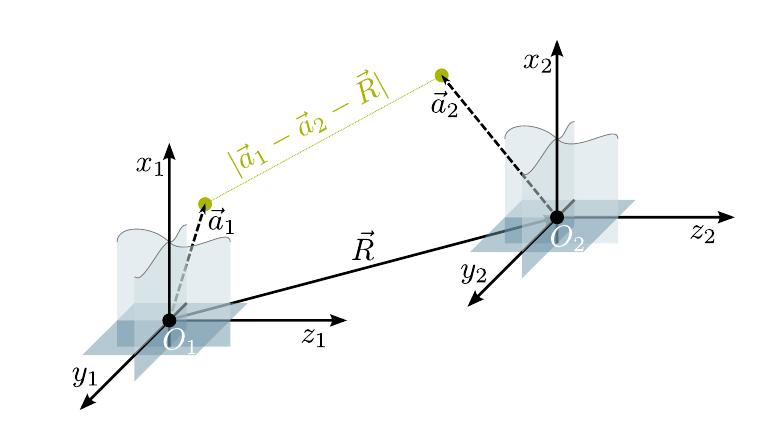
\includegraphics[scale=0.7]{bipolar}
    \centering 
    \caption{Scheme of two particles expanded according to two different origins [from ADD REFERENCE]}
    \label{fig:bipolar}
    \end{figure}




	
	\subsection{Workflow of the algorithm}
	
	Once some Mathematical preliminaries are set, it is possible to explain the workflow of the Algorithm.
	
	\subsubsection{Spliting the Space}
	
	The first step of the scheme is to split the space in order to generate different groups. The idea is to recursively split the space in eight octants, created the so-called structure of an \textit{octree}. So the number of boxes is $8^{D-1}$, where $D$ is the depth of the oct-tree.
	
		
	
	\begin{figure}[H]
	

    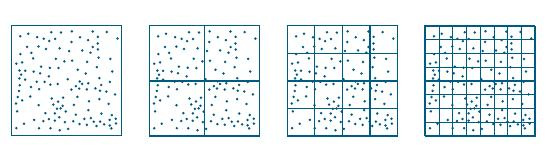
\includegraphics[scale=0.9]{BoxDepth}
    
    \centering
 
    \caption{Example of a division of the space in boxes. The following example is in 2D so the structure of the space is a \textit{quadtree}.}
    
    \label{fig:depth}
     \end{figure}
	
    
    The number of subdivisions is called the \textit{depth} $D$. For example, in figure \ref{fig:depth}, we can observe from left to right the depths $0,1,2$ and $3$.
    
    It is then possible to assign each particle of the simulation to the boxes of lowest depth.
    
    \subsubsection{Computing the Multipole moments}
    
    Once every particle is assigned to its box, we will compute the multipole moment $\omega_{lm}^j$ of each box.
    
    \begin{equation}
    \omega_{lm}^{j}(q,\textbf{a}) = q^j a_j^l \widetilde{P}_{lm}(\cos(\alpha_j))e^{-im\beta_j}
    \end{equation}
%
Then each multipole order can be moved to the Center of the box using the so-called $M2M$ (Multipole to Multipole) operator:    
    
    \begin{equation}
    \omega(\textbf{a} + \textbf{b}) = \sum\limits_{j=0}^{k} \sum\limits_{k=-j}^{j} \omega_{jk}(\textbf{a}) O_{l-j,m-k}(\textbf{b})
    \end{equation}

   $O_{l-j,m-k}(\textbf{b})$ is called the $M2M$ operator
   
   \begin{figure}[H]
   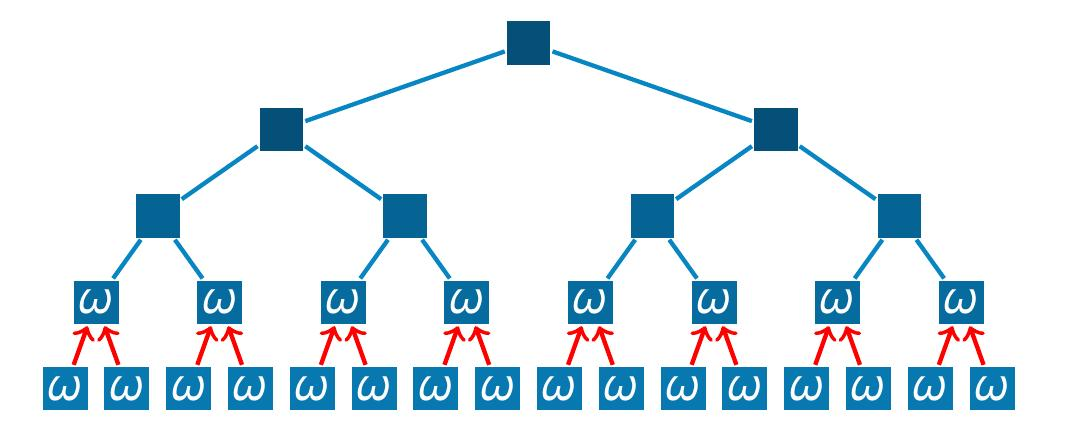
\includegraphics[scale=0.4]{ShiftMultipole}
    \centering 
    \caption{Example in 1-D showing the shifting of the multipole moments using the M2M operator. }
    \label{fig:ShiftMultipole}
   \end{figure}
   
   	\subsubsection{Transforming distant expansions into multipoles}
   	
   	



\chapter{Comparing FMM and PME accuracy}

    In this chapter I will more precfisely explain my work done in the Lab, which consisted in comparing the PME methods, which is for example used by gromacs, and the FMM mnethod, used by a solver made between the Julich Forschungszentrum and the Max Planck Institute for Biophysics in Göttingen.

    In will first explain for Gromacs work and then 


\section{Presentation of GROMACS}

    GROMACS (GROningen MAchine for Chemical Simulations) is a simulation software used for Molecular dynamics. It was originally developed in the Biophysical Chemistry department of University of Groningen but it is now develloped arround the world. GROMACS is made to be as fast as possible using all possible techniques to improve its performance (MPI, GPU computing) 
    
   
	\subsection{Structure of a File}
	
	 The program is used  by modifying text files that giving information on the structure of the system that has to be simulated and the parameters of the simulation. The files are the following 
	 
	\begin{itemize}
	
	\item The *.pdb file are the \textit{Protein DataBank} file : In this file is denoted the position and the type of the particles of the system. It also gives the size of the simulation box

	\item The *.top files (namelt \textit{topoloy} files) are the file where the properites of the atoms are defined. These properties are for example the charge, the Van-der-Waals parameters or the binding forces of the system. This configuration is often done with force field files such as AMBER or CHARMM
		 
	\item The *.mdp files are defining the physical and computational parameters of the simulation. It is defining the methods used for the simulation. In our case we are mostly interested in the electrostatics part of the computation ; it is then possible to select the method (PME or Cut-Off methods) and the parameters for the PME
	
	\end{itemize}
		
	\subsection{PME parameters}
	
	In this paragraph I will explain the parameters it is possible to play with:
	
	\begin{enumerate}
	

	\item[\textbf{CutOff}] The first parameter is the CutOff : It allows to set the Cut-Off radius for the Cut-Off method, but it also sets the difference between the direct part and the reciprocal part in the PME method
	
	\item[\textbf{Fourier Spacing}] The other important parameter is the fourier spacing. I remind that in the PME method a 3D FFT is done in order to compute the energies and the forces of the system. The FFT is so computed on a grid : The dimension of the grid is given by the \textit{Fourier Spacing} parameter.
	
	\item[\textbf{PME Order}] The PME order gives the order of the interpolation. For instance, PMEorder$= 4$ corresponds to a cubic interpolation. 		
	
	\end{enumerate}
	
\section{Presentation of fmsolvr}	




	
\section{Making GROMACS and fmsolvr comparable}	

\subsection{File manipulation}
\subsection{Adding Dipole correction to }



\section{Error plots}

\chapter*{Conclusion}

\nocite{*}
\bibliographystyle{plain}
\bibliography{biblio} 

\begin{appendices}
\chapter{Structure of Gromacs files}
The contents...
\end{appendices}



























\end{document}